\documentclass[aspectratio=169]{beamer}

\usetheme{default}
\usecolortheme{default}
\setbeamercolor{normal text}{fg=black,bg=white}
\setbeamercolor{frametitle}{fg=black}
\setbeamercolor{structure}{fg=black}
\setbeamertemplate{navigation symbols}{}
\setbeamertemplate{footline}{}

\usepackage{graphicx}
\usepackage{helvet}
\renewcommand{\familydefault}{\sfdefault}

\usepackage[T2A]{fontenc}
\usepackage[utf8]{inputenc}
\usepackage[russian]{babel}

\title{Gaphor}
\subtitle{UML SysML C4}
\date{}

\begin{document}

% --- 1 ---
\begin{frame}
\titlepage
\end{frame}

% --- 2 ---
\begin{frame}{О приложении}
Простое. Компактное. Кроссплатформенное.
\end{frame}

% --- 3 ---
\begin{frame}{Открытый проект}
Apache License 2.0 \\
Python + GTK \\
Windows / macOS / Linux \\
Разработка с 2019 года
\end{frame}

% --- 4 ---
\begin{frame}{Стартовый экран}
\centering
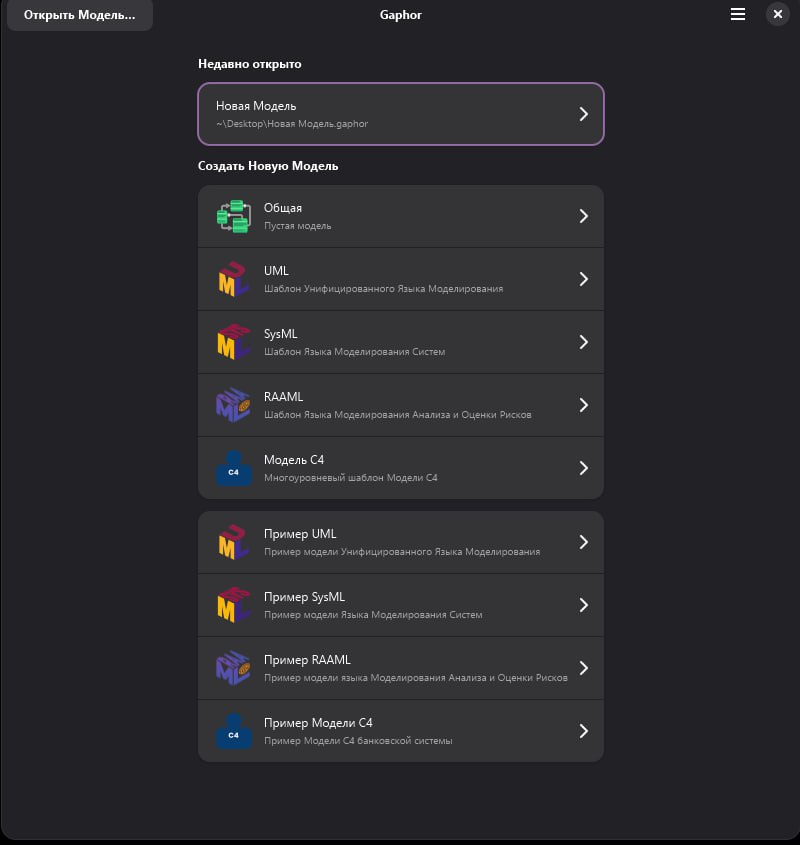
\includegraphics[width=\linewidth,height=0.8\textheight,keepaspectratio]{1.jpg}
\end{frame}

% --- 5 ---
\begin{frame}{SysML — «Модель навигации»}
\centering
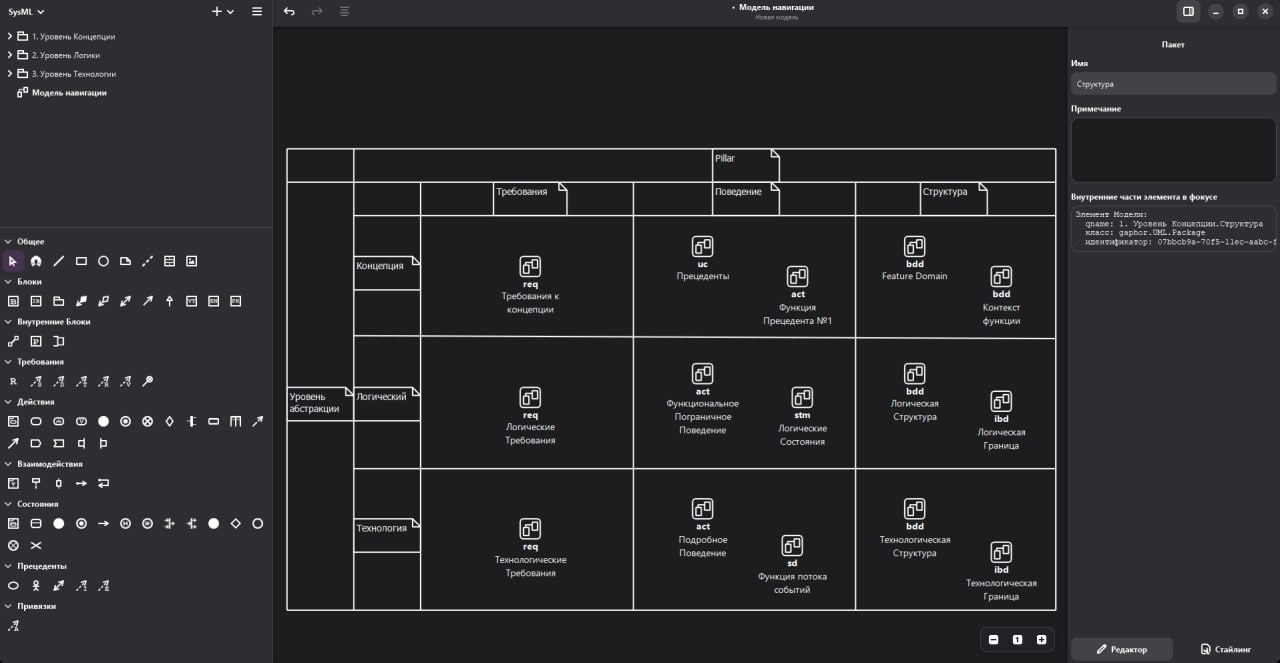
\includegraphics[width=\linewidth,height=0.8\textheight,keepaspectratio]{2.jpg}
\end{frame}

% --- 6 ---
\begin{frame}{UML — Классы автомобиля}
\centering
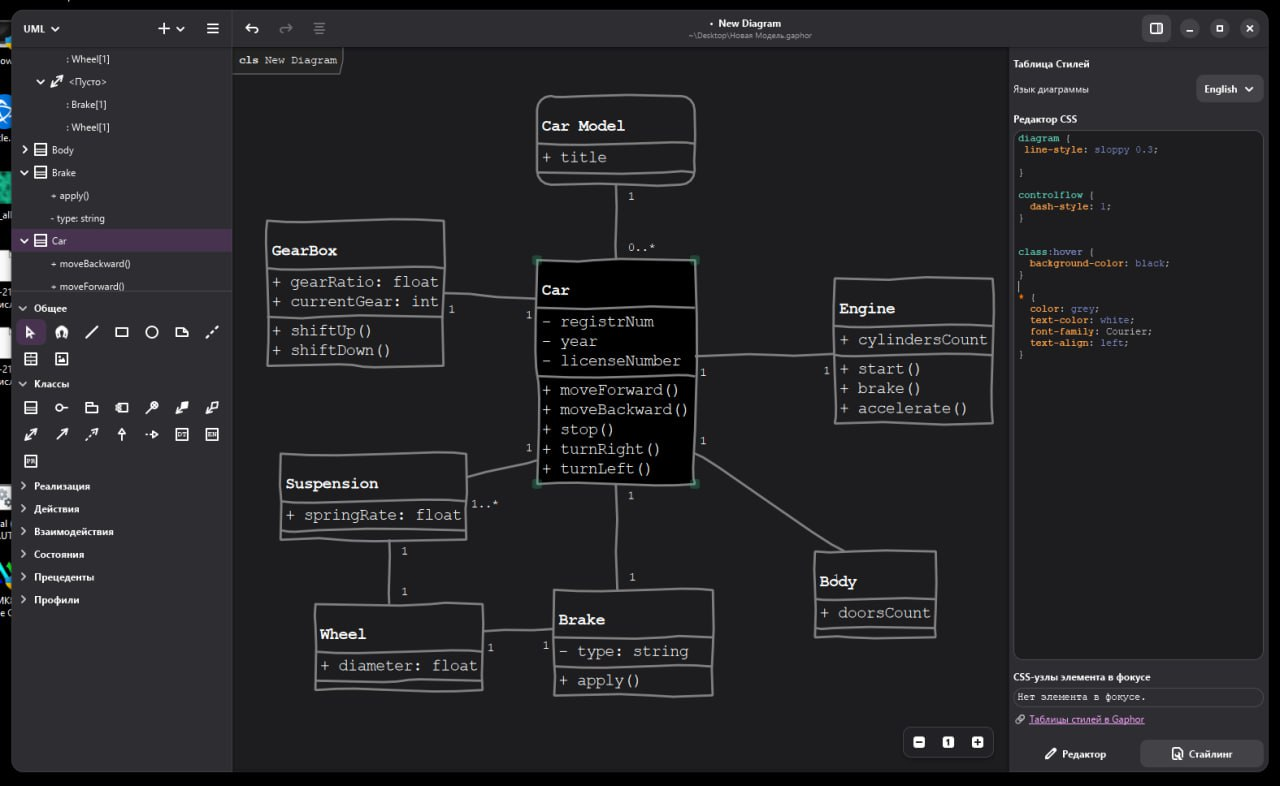
\includegraphics[width=\linewidth,height=0.8\textheight,keepaspectratio]{3.jpg}
\end{frame}

% --- 7 ---
\begin{frame}{Выбор языка моделирования}
\centering
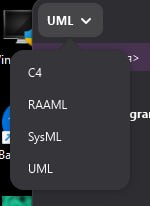
\includegraphics[width=\linewidth,height=0.8\textheight,keepaspectratio]{4.jpg}
\end{frame}

% --- 8 ---
\begin{frame}{Модули}
\centering
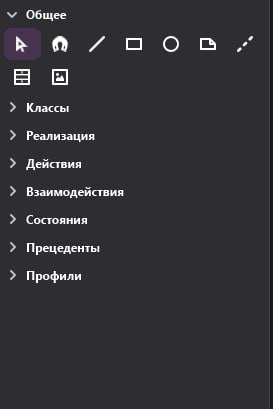
\includegraphics[width=\linewidth,height=0.8\textheight,keepaspectratio]{5.jpg}
\end{frame}

% --- 9 ---
\begin{frame}{Свойства класса}
\centering
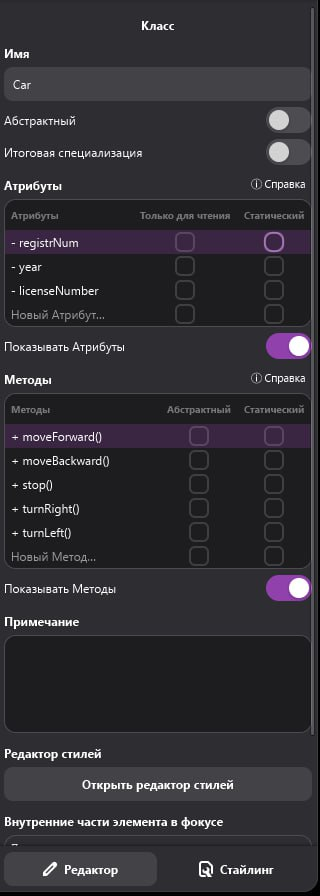
\includegraphics[width=\linewidth,height=0.8\textheight,keepaspectratio]{6.jpg}
\end{frame}

% --- 10 ---
\begin{frame}{Стайлинг (CSS)}
\centering
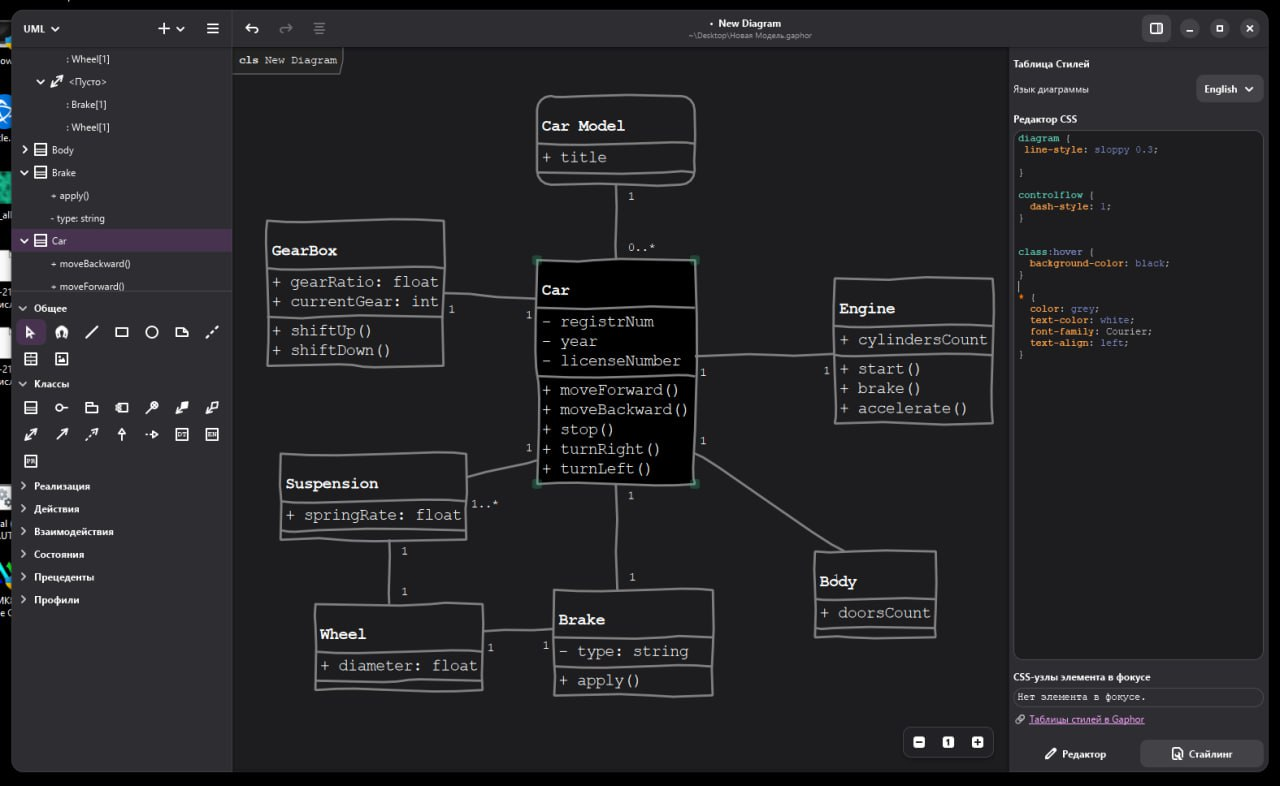
\includegraphics[width=\linewidth,height=0.8\textheight,keepaspectratio]{7.jpg}
\end{frame}

% --- 11 ---
\begin{frame}{Иерархия}
\centering
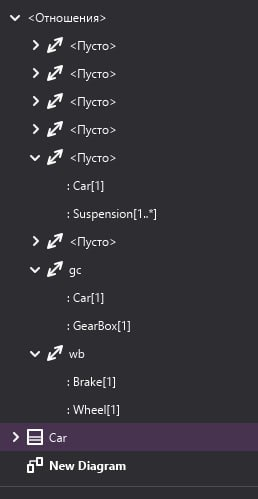
\includegraphics[width=\linewidth,height=0.8\textheight,keepaspectratio]{8.jpg}
\end{frame}

% --- 12 ---
\begin{frame}{Горячие клавиши}
\centering
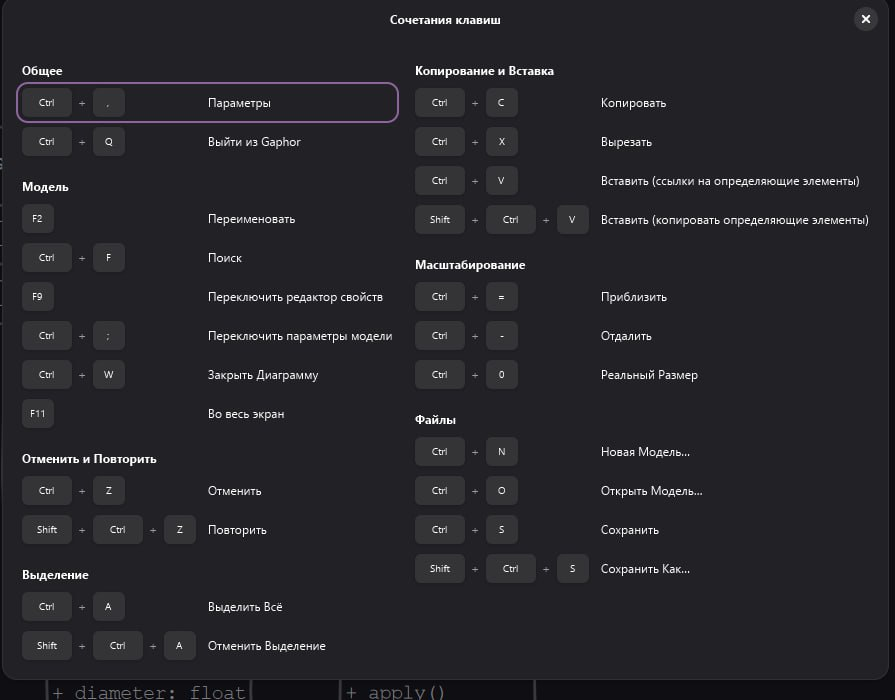
\includegraphics[width=\linewidth,height=0.8\textheight,keepaspectratio]{9.jpg}
\end{frame}

% --- 13 ---
\begin{frame}{Авторасположение}
\centering
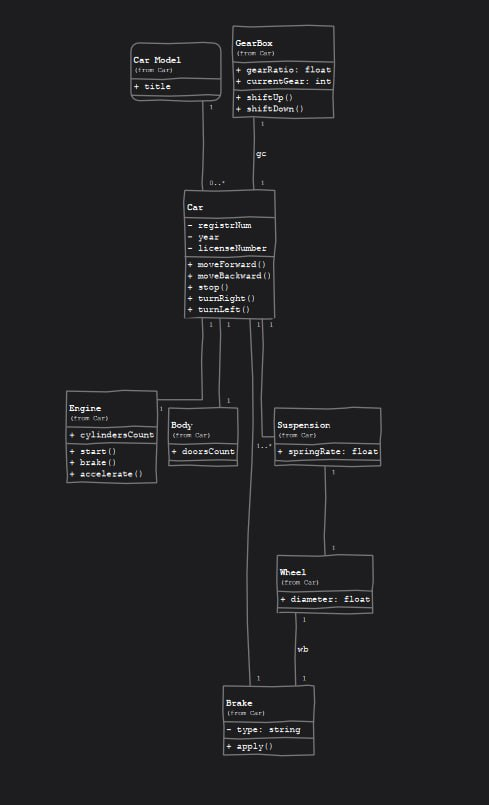
\includegraphics[width=\linewidth,height=0.8\textheight,keepaspectratio]{11.jpg}
\end{frame}

% --- 13 ---
\begin{frame}{Разработчики}
\centering
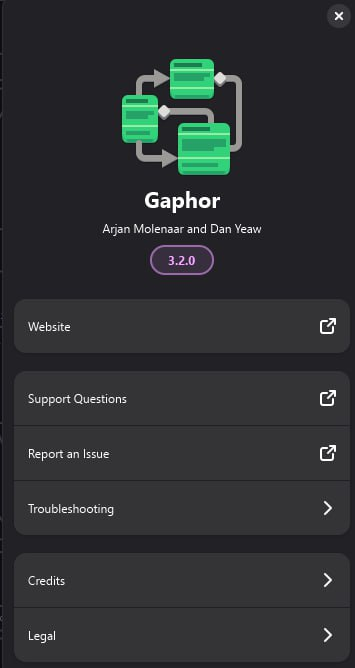
\includegraphics[width=\linewidth,height=0.8\textheight,keepaspectratio]{12.jpg}
\end{frame}


\end{document}
